\documentclass[11pt,a4paper]{article}
\usepackage[utf8]{inputenc}
\usepackage[T1]{fontenc}
\usepackage{amsmath,amssymb}
\usepackage[a4paper,margin=2.2cm]{geometry}
\usepackage{booktabs}
\usepackage{tabularx}
\usepackage{xcolor}
\usepackage{parskip}
\usepackage{titlesec}
\usepackage{enumitem}
\usepackage{graphicx}
\usepackage{float}

\definecolor{NavyBlue}{HTML}{0b4f9e}
\usepackage[colorlinks=true,linkcolor=NavyBlue,urlcolor=NavyBlue,citecolor=NavyBlue]{hyperref}

\titleformat{\section}{\large\bfseries}{\thesection.}{0.6em}{}
\titleformat{\subsection}{\normalsize\bfseries}{\thesubsection}{0.6em}{}
\newcolumntype{L}{>{\raggedright\arraybackslash}X}
\newcommand{\code}[1]{\texttt{\small #1}}
\newcommand{\op}[1]{\texttt{\small #1}}
\definecolor{cpass}{HTML}{1a7f37}
\definecolor{cfail}{HTML}{cf222e}
\definecolor{cskip}{HTML}{8b949e}
\newcommand{\gpass}[1]{\textcolor{cpass}{\textbf{#1}}}
\newcommand{\gfail}[1]{\textcolor{cfail}{\textbf{#1}}}
\newcommand{\gskip}[1]{\textcolor{cskip}{#1}}

% GENERATED by gates.py -- do not edit
\newcommand{\tblGates}{%
{\scriptsize\setlength{\tabcolsep}{4pt}
\begin{tabularx}{\textwidth}{@{}llLllL@{}}\toprule
& \textbf{gate} & \textbf{threshold} & \textbf{measured} & \textbf{outcome} & \textbf{figure}\\\midrule
\multicolumn{6}{@{}l}{\textit{bookkeeping --- does the code do what the operator says?}}\\
G1 & all four options PARSE (24 combinations) & 24 of 24 option combinations load & 24 & \gpass{PASS} & {\tiny \href{log/toy_wave_noed_simple_p1_free/G1_options.png}{G1\_options.png}}\\
G1b & all four options BUILD and take one step & 24 of 24 option combinations run one forward step & --- & \gskip{SKIP} & {\tiny ---}\\
G2 & nothing dataset-specific is hardcoded & 0 offending literals outside config/ & 0 & \gpass{PASS} & {\tiny \href{log/toy_wave_noed_simple_p1_free/G2_scan.png}{G2\_scan.png}}\\
G3 & scatter-$>$gather round trip on a constant field & $<$ 1e-6 of the field value & --- & \gskip{SKIP} & {\tiny ---}\\
G4 & transfer weights are a partition of unity & $|$sum(w) - 1$|$ $<$ 1e-6 & --- & \gskip{SKIP} & {\tiny ---}\\
G5 & simple + 1 pass + no enc/dec is arithmetically NeuralGNN & $<$ 1e-5 of the voltage range & --- & \gskip{SKIP} & {\tiny ---}\\
G6 & residual blocks start at identity: 1 vs 16 passes at init & bit-identical (max $|$delta$|$ == 0) & --- & \gskip{SKIP} & {\tiny ---}\\
G7 & units declared, and every measurement threshold is in phenomenon units & 1 = declared and checked & 1 & \gpass{PASS} & {\tiny \href{log/toy_wave_noed_simple_p1_free/G7_units.png}{G7\_units.png}}\\
G8 & a K=20 rollout on the toy does not diverge & state norm stays $<$ 2x the ground-truth norm & --- & \gskip{SKIP} & {\tiny ---}\\
\multicolumn{6}{@{}l}{\textit{closed form --- does it reproduce the physics it was given?}}\\
G9 & recover the spatial interaction kernel (toy\_small) & R\^{}2 $>$ 0.90 against the GT kernel & --- & \gskip{SKIP} & {\tiny ---}\\
G10 & recover per-type time constants, GT graph supplied & R\^{}2 $>$ 0.95 against the known tau & --- & \gskip{SKIP} & {\tiny ---}\\
G11 & a\_i recovers the types (toy\_small) & ARI $>$ 0.70 against the 8 true types & --- & \gskip{SKIP} & {\tiny ---}\\
G12 & a\_i recovers the types (toy\_large) & ARI $>$ 0.70 against the 65 true types & --- & \gskip{SKIP} & {\tiny ---}\\
G13 & recover the per-neuron stimulus gain b\_i & R\^{}2 $>$ 0.90 against the true gain & --- & \gskip{SKIP} & {\tiny ---}\\
G14 & encoder/decoder is a genuine option: on vs off & $|$delta R\^{}2(kernel)$|$ $<$ 0.03 & --- & \gskip{SKIP} & {\tiny ---}\\
G15 & graphcast vs simple message is RESOLVED, either way & $|$delta$|$ reported against the 3-seed floor; below it is UNRESOLVED, not ranked & --- & \gskip{SKIP} & {\tiny ---}\\
G16 & types are spatially mixed by construction & spatial-cell type purity within 20\% of chance (1/n\_types) & 1.131 & \gpass{PASS} & {\tiny \href{log/toy_wave_noed_simple_p1_free/G16_toy.png}{G16\_toy.png}, \href{log/toy_wave_noed_simple_p1_free/G16_state.mp4}{G16\_state.mp4}}\\
G21 & the coarse field is a travelling wave, cyclic left to right & phase drift per frame within 5\% of lambda/period & 0.005224 & \gpass{PASS} & {\tiny \href{log/toy_wave_noed_simple_p1_free/G21_field.mp4}{G21\_field.mp4}}\\
G22 & the fine rule is exactly recoverable from (v, grad u) & minimum per-node R\^{}2 $>$ 0.90 & 0.9981 & \gpass{PASS} & {\tiny \href{log/toy_wave_noed_simple_p1_free/G22_identifiability.png}{G22\_identifiability.png}}\\
G23 & the gradient is reconstructible from neighbours' states & R\^{}2 $>$ 0.95, else the graph cannot carry the fine rule & 1 & \gpass{PASS} & {\tiny \href{log/toy_wave_noed_simple_p1_free/G22_identifiability.png}{G22\_identifiability.png}}\\
G24 & the heterogeneity is linearly readable & corr(fitted gain, true g\_i) $>$ 0.90 & 0.9807 & \gpass{PASS} & {\tiny \href{log/toy_wave_noed_simple_p1_free/G24_heterogeneity.png}{G24\_heterogeneity.png}}\\
G25 & connected nodes are not collinear & mean $|$corr$|$ between connected nodes $<$ 0.80 & 0.6074 & \gpass{PASS} & {\tiny \href{log/toy_wave_noed_simple_p1_free/G22_identifiability.png}{G22\_identifiability.png}}\\
\multicolumn{6}{@{}l}{\textit{measurement --- does it agree with something observed?}}\\
G17 & ZAPBench held-out prediction of d(dF/F)/dt & R\^{}2 $>$ 0.268, the parameter-free kNN spatial pool & --- & \gskip{SKIP} & {\tiny ---}\\
G18 & the learned stimulus gain b\_i is spatially structured & Moran's I $>$ 0.2 over the soma graph, against a permutation null & --- & \gskip{SKIP} & {\tiny ---}\\
G19 & fitted calcium decay time constant & 0.5 - 2 s (GCaMP6) & --- & \gskip{SKIP} & {\tiny ---}\\
G20 & redox field fit reproduces the washout response & THRESHOLD TO BE FIXED from Development\_Time\_Trend.xlsx, before the run & --- & \gskip{SKIP} & {\tiny ---}\\
\bottomrule\end{tabularx}}}
\newcommand{\gateFigures}{%
\begin{figure}[htbp]\centering

\includegraphics[width=\linewidth]{log/toy_wave_noed_simple_p1_free/G1_options.png}
\caption{\textbf{G1} --- all four options PARSE (24 combinations). Threshold: 24 of 24 option combinations load. Measured: 24. Outcome: PASS.}
\end{figure}
\begin{figure}[htbp]\centering

\includegraphics[width=\linewidth]{log/toy_wave_noed_simple_p1_free/G2_scan.png}
\caption{\textbf{G2} --- nothing dataset-specific is hardcoded. Threshold: 0 offending literals outside config/. Measured: 0. Outcome: PASS.}
\end{figure}
\begin{figure}[htbp]\centering

\includegraphics[width=\linewidth]{log/toy_wave_noed_simple_p1_free/G7_units.png}
\caption{\textbf{G7} --- units declared, and every measurement threshold is in phenomenon units. Threshold: 1 = declared and checked. Measured: 1. Outcome: PASS.}
\end{figure}
\begin{figure}[htbp]\centering

\includegraphics[width=\linewidth]{log/toy_wave_noed_simple_p1_free/G16_toy.png}
\caption{\textbf{G16} --- types are spatially mixed by construction. Threshold: spatial-cell type purity within 20\% of chance (1/n\_types). Measured: 1.131. Outcome: PASS.}
\end{figure}
\noindent\small G16 also has a movie: \href{log/toy_wave_noed_simple_p1_free/G16_state.mp4}{G16\_state.mp4}.\par\medskip
\begin{figure}[htbp]\centering
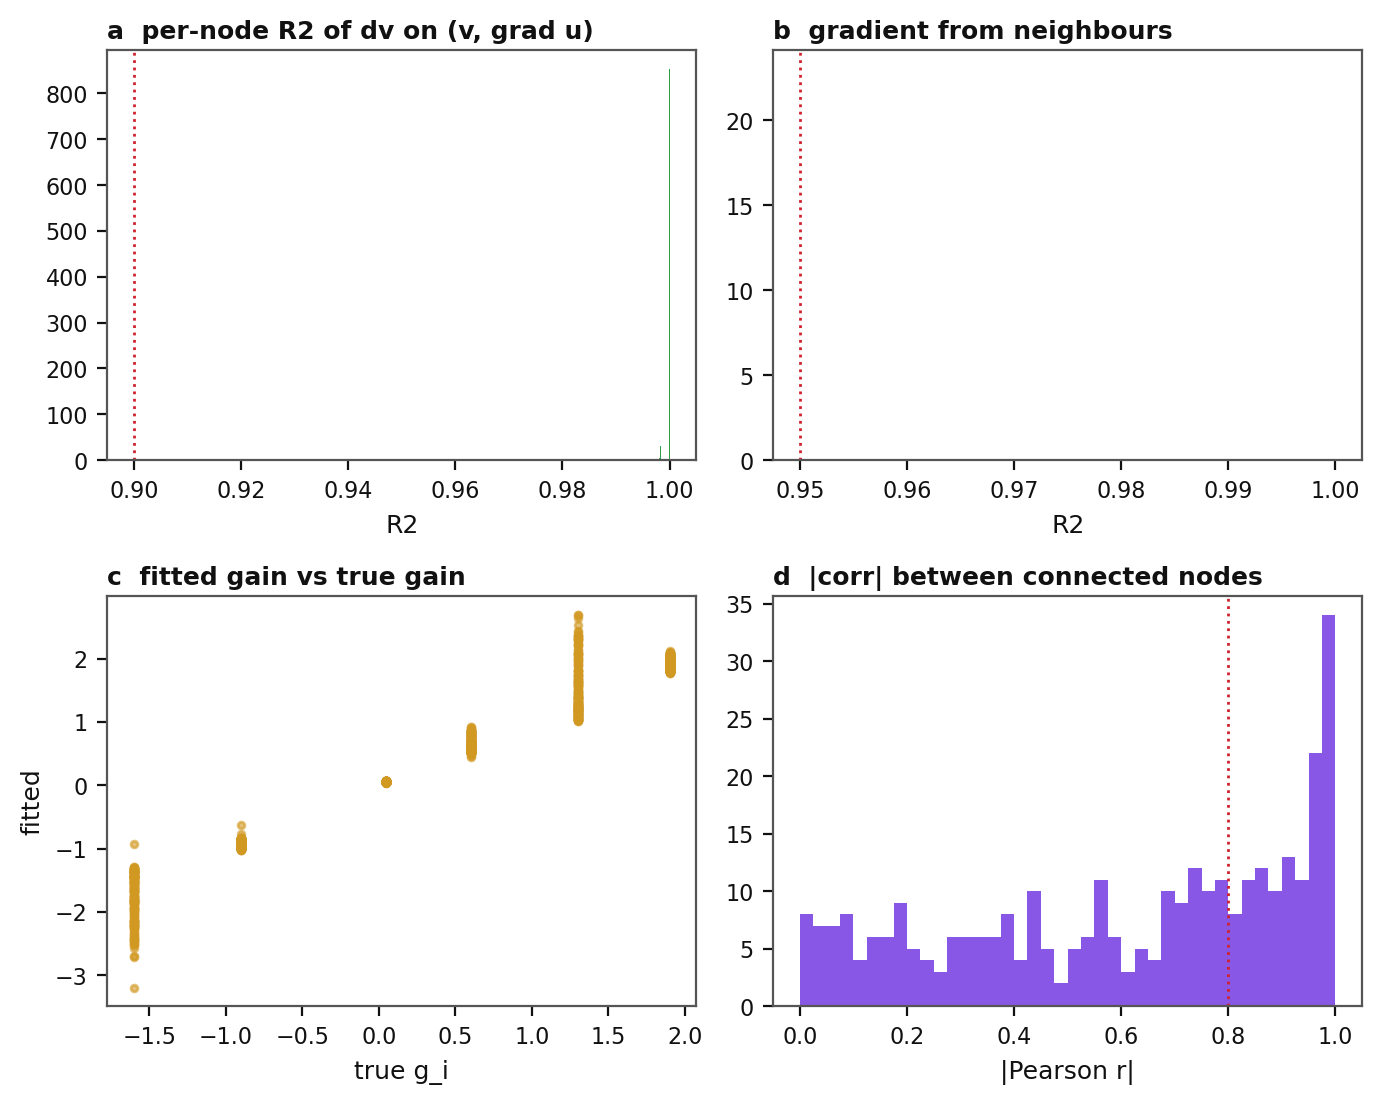
\includegraphics[width=\linewidth]{log/toy_wave_noed_simple_p1_free/G22_identifiability.png}
\caption{\textbf{G22} --- the fine rule is exactly recoverable from (v, grad u). Threshold: minimum per-node R\^{}2 $>$ 0.90. Measured: 0.9981. Outcome: PASS.}
\end{figure}
\begin{figure}[htbp]\centering
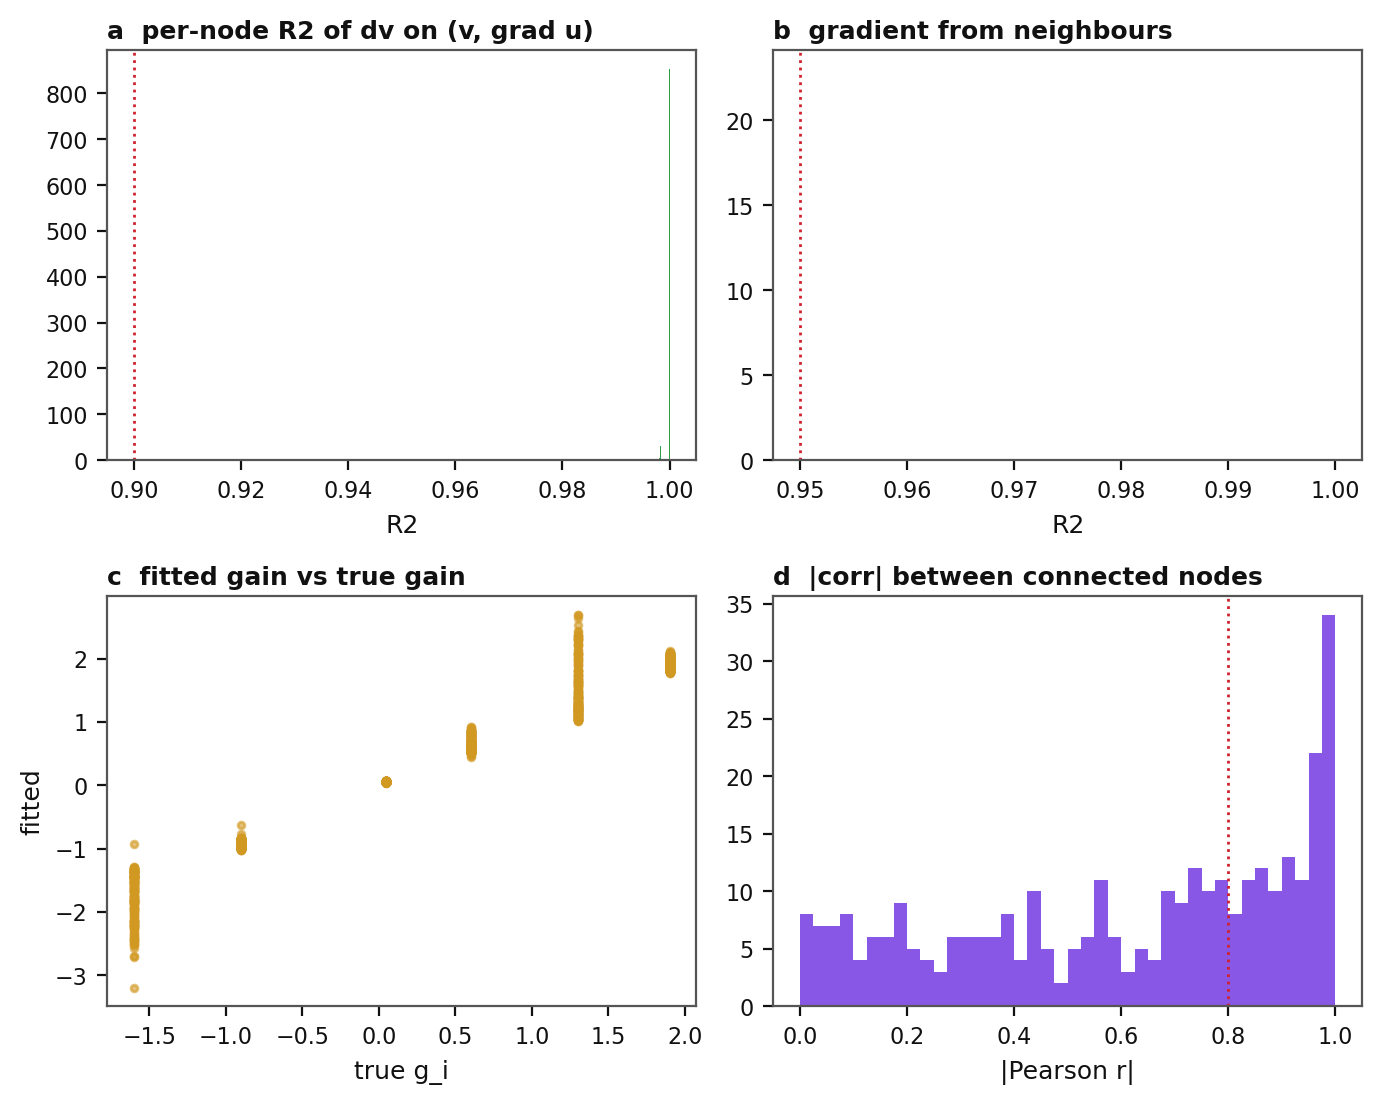
\includegraphics[width=\linewidth]{log/toy_wave_noed_simple_p1_free/G22_identifiability.png}
\caption{\textbf{G23} --- the gradient is reconstructible from neighbours' states. Threshold: R\^{}2 $>$ 0.95, else the graph cannot carry the fine rule. Measured: 1. Outcome: PASS.}
\end{figure}
\begin{figure}[htbp]\centering
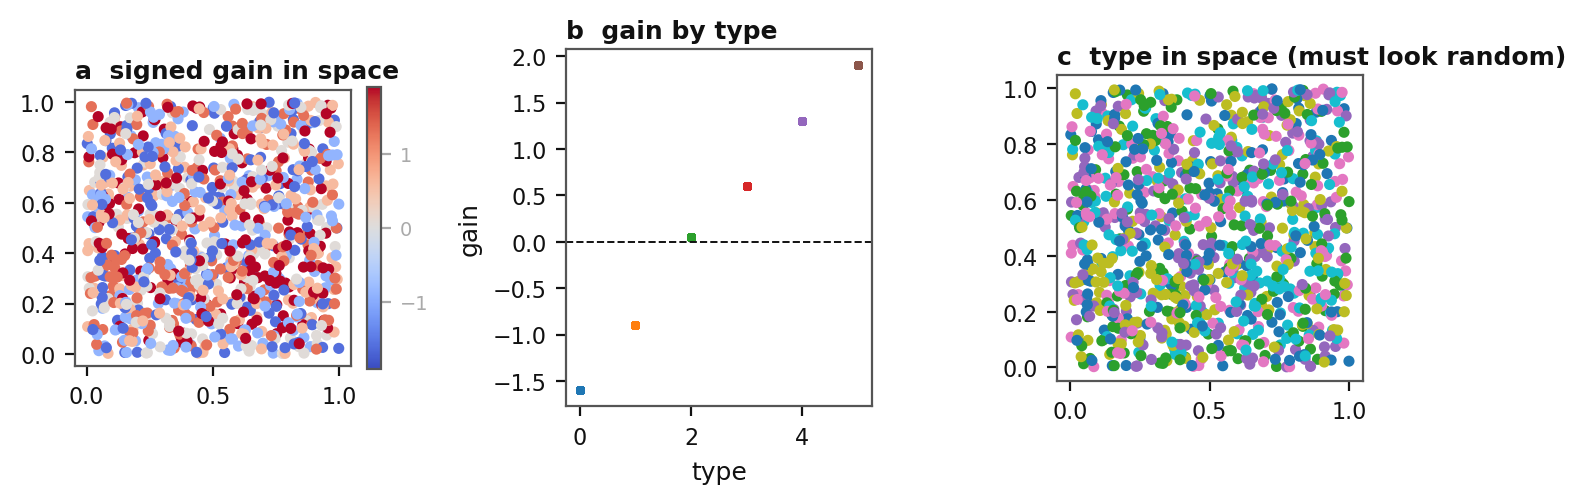
\includegraphics[width=\linewidth]{log/toy_wave_noed_simple_p1_free/G24_heterogeneity.png}
\caption{\textbf{G24} --- the heterogeneity is linearly readable. Threshold: corr(fitted gain, true g\_i) $>$ 0.90. Measured: 0.9807. Outcome: PASS.}
\end{figure}
\begin{figure}[htbp]\centering
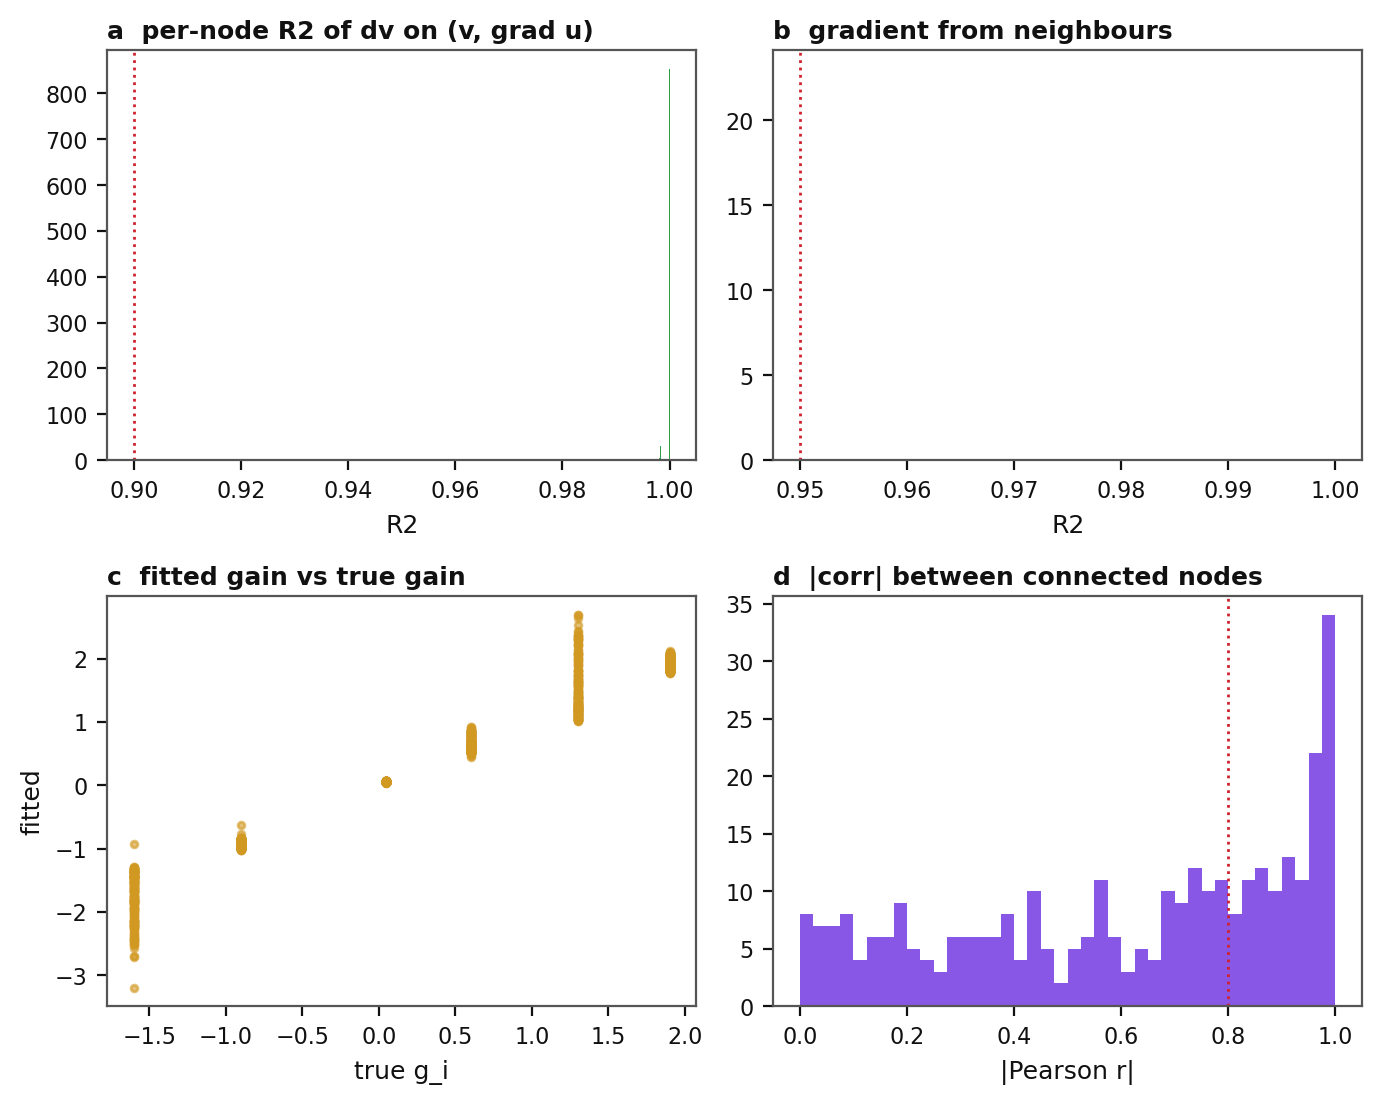
\includegraphics[width=\linewidth]{log/toy_wave_noed_simple_p1_free/G22_identifiability.png}
\caption{\textbf{G25} --- connected nodes are not collinear. Threshold: mean $|$corr$|$ between connected nodes $<$ 0.80. Measured: 0.6074. Outcome: PASS.}
\end{figure}
}
\newcommand{\tierProportion}{9 bookkeeping / 13 closed form / 4 measurement}


\title{\bfseries A GraphCast-style fitting model as Plexus2 operators\\[3pt]
\large Stages 0--1b: the container, the two-scale toy, and the gates it must pass}
\author{\code{Plexus/prototype/graphcast} --- prototype only, nothing promoted}
\date{2026-08-30}

\begin{document}
\maketitle

\begin{abstract}
\noindent
This prototype expresses a GraphCast-style dynamics model as a composition of Plexus2 sets, fields
and operators, so that one spec language covers a toy with ground truth, a point-cloud recording
and a field recording. Four architectural choices --- an encoder/decoder through a background grid,
the message form, the number of message-passing passes, and the node embedding --- are
\emph{configuration options} rather than forks, giving $24$ legal combinations from one
implementation. This note covers stages 0 to 1b: the container, the two-scale toy, and the nine
gates now passing. \textbf{No model has been gated yet}, and that is deliberate: three successive
toys failed for reasons that had nothing to do with any model, and stage 1b exists because in each
case training had been run before the data was known to pose the problem it claimed to.
\end{abstract}

\section{Mechanism}

Every model in \code{connectome-gnn} is a one-step message-passing network on a \emph{given}
connectome. Two things wanted now sit outside that: a deeper, edge-stateful processor, and datasets
with no connectome at all. The zebrafish recording has $71{,}721$ neurons of which about $481$ are
matched to an electron-microscopy reconstruction; the organoid is a three-dimensional field with no
segmentation. In both, the coupling has to come from \emph{space} rather than from wiring.

\paragraph{The arithmetic that decides what can be represented.} A zebrafish volume is acquired
plane by plane --- $72$ planes at $12.0$\,ms, so one volume takes $0.851$\,s against a $0.914$\,s
frame interval, which is $93\%$ of the frame period. Neurons at different depths are therefore
\emph{not} sampled simultaneously, and simultaneity is exactly what a message-passing operator
assumes. That is a fact about the data rather than a modelling choice; the per-plane acquisition
times are recorded, so the model can be conditioned on the offset rather than pretending it away.

\paragraph{The toy is two scales with deliberately different rules.} A test bed whose coarse and
fine mechanisms are the same rule at two resolutions cannot show whether a multi-scale operator is
doing anything at all. So:

\begin{center}
\begin{tabularx}{\textwidth}{@{}p{1.9cm}p{3.3cm}L@{}}
\toprule
\textbf{scale} & \textbf{operator} & \textbf{rule} \\
\midrule
coarse & \op{wave\_field} & a wave travelling cyclically left to right; one rule, no per-node
  freedom \\
fine & \op{gradient\_gain} & each node amplifies the \emph{local gradient} of that field with its
  own \emph{signed} gain \\
\bottomrule
\end{tabularx}
\end{center}

\noindent
The heterogeneity lands in the fine rule, as a signed per-node gain: some nodes amplify the
gradient, others invert it. Unlike a time constant, that cannot be read off a node's own trace
without reference to the field around it --- which is what makes the graph load-bearing rather than
a small correction to a mostly-local law.

\section{Equations and symbols}

\begin{align}
\textbf{coarse:}\quad & \frac{\partial u}{\partial t} + c\,\frac{\partial u}{\partial x} = 0 ,
\qquad
u(x,t) = A \sin\!\Big(2\pi\Big(\frac{x}{\lambda} - \frac{t}{T}\Big)\Big) ,
\qquad c = \frac{\lambda}{T}
\label{eq:coarse}\\[4pt]
\textbf{fine:}\quad & \frac{\mathrm{d}v_i}{\mathrm{d}t}
   = -\frac{v_i}{\tau_i} \;+\; g_i \,\frac{\partial u}{\partial x}(\mathbf{r}_i)
\label{eq:fine}
\end{align}

The coarse field is written in closed form rather than stepped, and that is deliberate: it is the
exact solution of \eqref{eq:coarse}, so the coarse scale carries no discretisation error of its own
that could later be mistaken for an error in the rule under test.

\begin{center}
\begin{tabularx}{\textwidth}{@{}p{1.4cm}p{2.6cm}L@{}}
\toprule
\textbf{symbol} & \textbf{units} & \textbf{what it is \emph{of}} \\
\midrule
$u(x,t)$ & field units & the coarse field, one scalar per point of the domain \\
$A$ & field units & wave amplitude \\
$\lambda$ & length & wavelength, \emph{as a fraction of the domain width} \\
$T$ & frames & wave period, in simulation frames \\
$c = \lambda/T$ & length\,/\,frame & phase speed --- the quantity gate G21 measures \\
$v_i$ & state units & the state of node $i$; the observable \\
$\tau_i$ & time & node $i$'s time constant, a per-\emph{type} constant \\
$g_i$ & state\,/\,(field\,/\,length) & node $i$'s \textbf{signed gain} on the field gradient ---
  the heterogeneity \\
$\mathbf{r}_i$ & length & node $i$'s position, fixed \\
\bottomrule
\end{tabularx}
\end{center}

\noindent
$\tau_i$ and $g_i$ are intensive: properties of a node rather than sums over it, so neither changes
if the node set is resampled at a different density. That matters because the same operators are
meant to run on $1{,}024$ toy nodes and on $71{,}721$ real ones.

\section{The Plexus2 container}

\begin{center}
\begin{tabularx}{\textwidth}{@{}p{2.7cm}p{1.8cm}p{2.4cm}L@{}}
\toprule
\textbf{operator} & \textbf{kind} & \textbf{acts on} & \textbf{mechanism} \\
\midrule
\op{wave\_field} & \code{field} & field \code{u} & Eq.~\eqref{eq:coarse}; prescribed, exact \\
\op{gradient\_gain} & \code{exchange} & \code{neuron} $\leftarrow$ \code{u} &
  Eq.~\eqref{eq:fine}; \code{EMIT = velocity}, so the engine integrates it \\
\bottomrule
\end{tabularx}
\end{center}

\noindent
Both are prototype-local, registered through the ordinary \code{@register\_operator} decorator;
nothing is written into \code{src/plexus/}. The forward run is \code{plexus.engine.run} unchanged,
and the interaction graph is built from the node positions by the \emph{fit}, never by the
generator --- building the generator on the same graph the model is given would hand it the answer.

\paragraph{The four options.} \code{encoder\_decoder} (\code{off}\,/\,\code{on}), \code{message}
(\code{simple}\,/\,\code{graphcast}), \code{n\_passes} ($\geq 1$), and \code{embedding}
(\code{none}\,/\,\code{free}\,/\,\code{multires}). The schema refuses \code{simple} at more than
one pass --- that form carries no edge state, so repeating it is a different model from the one it
claims to be --- which leaves $2 \times 4 \times 3 = 24$ legal combinations, the count G1 checks.

\paragraph{Where the training scheme comes from.} The optimiser follows GraphCast where its choices
are measured (AdamW with $\beta_2 = 0.95$, a global gradient-norm clip, a linear warmup then cosine
decay \emph{to zero}, and the target normalised by the inverse variance of the \emph{increment}
rather than of the state), and \code{connectome-gnn}'s production configs elsewhere: a separate
learning rate for the interaction weights, $L_1$ and $L_2$ on those weights, a Lipschitz smoothness
prior on the message function, and a group lasso over the message's input blocks. The last was
measured in the weekend benchmark to recover $+0.153$ in $R^2_W$ on five of five folds by removing
a degeneracy rather than by preferring simpler models --- which is why accuracy rose rather than
trading off. The rollout knobs the same benchmark separated (horizon schedule, truncation window,
shooting stride, step weighting) are implemented so its finding --- that plain one-step training
wins --- can be reproduced here rather than assumed.

\section{Gates}

A gate is a number with a threshold decided \emph{before} the run and a stated consequence if it
fails. A threshold chosen after seeing the number is not a threshold, so every threshold is a
literal in \code{gates.py} and predates the code it gates. This table is \tierProportion, so two
thirds of it is verification rather than validation. That is the expected shape and is stated
rather than hidden.

A gate's threshold belongs in the unit of the phenomenon, not of the mesh: a threshold in grid
cells is denominated in the currency in which it is easiest to pass, and a green row of that kind
reads as an endorsement the model has not earned. Every row therefore carries what its number is
\emph{of}, and the measurement tier is available only because the spec declares
\code{general.units:}. \textbf{An artifact is a condition of passing} --- a gate with no figure is
reported \gskip{SKIP}, never \gpass{PASS}.

\smallskip
\tblGates

\subsection{What the gates license, and what they do not}

Stages 0 and 1b have run. G1, G2 and G7 establish that all $24$ option combinations parse, that no
dataset path, name or dimension appears anywhere in the prototype's code, and that the spec
declares its units --- so the measurement-tier rows are \emph{available} to be denominated in
seconds and micrometres rather than in cells. G16 and G21--G25 establish that the toy is a valid
test bed: the coarse field really is a travelling wave at the speed asked for, the fine rule is
exactly recoverable from the state and the gradient, the gradient is reconstructible from a node's
neighbours, the heterogeneity is linearly readable, and connected nodes are not collinear.

\textbf{Nothing about any model is licensed.} Every gate on a fitted model is still \gskip{SKIP}.
G5 is the one to watch: it establishes that the \code{simple} option is arithmetically the existing
\code{NeuralGNN}, and therefore that everything after it is a controlled variation on something
already known to work rather than a new model whose failures cannot be attributed.

\subsection{Two gates failed first, and both failures were worth having}

\begin{itemize}[leftmargin=1.3em,itemsep=4pt]
\item \textbf{G25 at $0.841$ was a real defect.} With $\lambda = 0.5$, a twelve-neighbour
neighbourhood spans only $0.5$ radians of phase, so neighbours were very nearly redundant --- which
is precisely why an earlier fit drove the loss to $0.005$ while recovering none of the mechanism.
Shortening to $\lambda = 0.15$ moved it to $0.607$.
\item \textbf{G21 at $0.094$, then $0.053$, was the estimator twice over.} Taking the wave peak by
\code{argmax} on a $128$-cell grid quantises to whole cells while the wave moves about half a cell
per frame; replacing that with an FFT then used integer bin $7$ where the true mode is
$1/\lambda = 6.67$, biasing the speed by exactly $6.67/7 = 0.952$ --- which was the $5\%$ it
reported. Projecting onto the known wavelength gives $0.5\%$ error. \emph{An estimator has to be
sharper than the threshold it is judged against.}
\end{itemize}

\noindent
A third defect never reached a gate because a figure caught it first: nodes were spawned as a disc
about a randomly placed parent, so $58.8\%$ of them sat \emph{outside} the field domain, where
sampling clamps and the gradient is identically zero. The correlation between a node's fit quality
and its distance from the domain edge was $0.863$, which is what pointed at it.

\section{The evidence}

Every gate points to a figure, because the failures this prototype is most exposed to are visible
and not scalar. Three defects in earlier toys were each a plausible-looking number: a circuit
sitting at a fixed point (spatial spread $9.29$ against a temporal spread of $0.065$), a stimulus
field that was \emph{identically zero} for three generations because an operator read a clock that
nothing was writing, and a spatial type purity of $6.1\times$ chance that was the grid being finer
than the sampling. All three are obvious in a panel and invisible in a table.

\gateFigures

\end{document}
